\documentclass{article}
\usepackage{tikz}

\begin{document}

\begin{figure}[h]
    \centering
    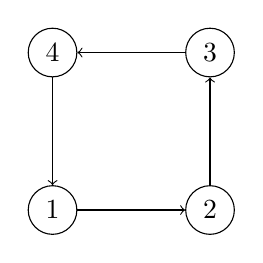
\begin{tikzpicture}
        % Define nodes
        \node[circle, draw] (A) at (0,0) {1};
        \node[circle, draw] (B) at (2,0) {2};
        \node[circle, draw] (C) at (2,2) {3};
        \node[circle, draw] (D) at (0,2) {4};

        % Draw edges
        \draw[->] (A) -- (B);
        \draw[->] (B) -- (C);
        \draw[->] (C) -- (D);
        \draw[->] (D) -- (A);

        % Add labels if needed
        % \node at (1,-0.5) {Label A};
        % \node at (3,0.5) {Label B};
        % \node at (3,2.5) {Label C};
        % \node at (-0.5,2.5) {Label D};
    \end{tikzpicture}
    \caption{A 4-Vertex Cycle Graph}
\end{figure}

\end{document}